
\documentclass[journal]{IEEEtran}

\usepackage{cite}

\usepackage{booktabs}


\ifCLASSINFOpdf
\usepackage{graphicx}
\graphicspath{Figures}
\else
\usepackage{graphicx}
\graphicspath{Figures}
\fi

% *** MATH PACKAGES ***
\usepackage{amsmath}
\interdisplaylinepenalty=2500

% *** SUBFIGURE PACKAGES ***
\ifCLASSOPTIONcompsoc
 \usepackage[caption=false,font=normalsize,labelfont=sf,textfont=sf]{subfig}
\else
  \usepackage[caption=false,font=footnotesize]{subfig}
\fi

\usepackage{color, colortbl}
\definecolor{Gray}{gray}{0.9}

\hyphenation{op-tical net-works semi-conduc-tor}


\begin{document}

\title{Layout Based Ultra-Fast Short-Circuit Protection Technique for Parallel~Connected GaN HEMTs}

\author{Furkan~Karakaya,~\IEEEmembership{Student Member,~IEEE,}
        Ozturk~Sahin~Alemdar,~\IEEEmembership{Student Member,~IEEE}
        and~Ozan~Keysan,~\IEEEmembership{Member,~IEEE}% <-this % stops a space
\thanks{The authors are with the METU PowerLab, Electrical and Electronics Engineering Department of Middle East Technical University, Ankara, Turkey (e-mail: \email{keysan@metu.edu.tr}).}
}


\markboth{Journal of \LaTeX\ Class Files,~Vol.~14, No.~8, August~2015}%
{Shell \MakeLowercase{\textit{et al.}}: Bare Demo of IEEEtran.cls for IEEE Journals}


\maketitle
\begin{abstract}

Gallium Nitride Enhancement-Mode High Electron Mobility Transistors (GaN HEMTs) help to achieve high power density converter circuits thanks to their superior efficiency, higher switching speed and small package size.
However, increased switching speed results in a sharp increase in short circuit (SC) current under a shoot-through fault with respect to other type of devices. GaN HEMTs can withstand the SC current only for several hundred nanoseconds. Therefore, fast SC protection solutions are critical for protecting power circuits.

In this paper, the voltage induced by high slew rate of SC current on the high frequency power loop inductance resulting from the printed circuit board (PCB) layout is sensed to implement an ultra-fast short-circuit protection technique.

The proposed technique does not increase circuit parasitics and provides flexibility in layout design that makes it suitable for parallel connected GaN HEMTs, which require symmetric layout design for equal current sharing.

A multi-pulse test is conducted under 1.56~MHz switching frequency, 400~VDC bus voltage and 40~A load current by using parallel connected GaN HEMTs in a half-bridge configuration to verify the robustness and reliability of the proposed protection technique.
Experimental results show that the proposed protection technique is able to detect SC fault within 40~ns and fault is completely cleared with a soft turn-off in 250~ns.

\end{abstract}

\begin{IEEEkeywords}
Circuit faults,
Gallium Nitride,
GaN HEMTs,
Transistor paralleling,
Layout design,
Short circuit protection
\end{IEEEkeywords}

\IEEEpeerreviewmaketitle

\section{Introduction}
\label{sec_intro}
\IEEEPARstart{C}{urrent} trend in power electronics is to increase efficiency and reduce volume without sacrificing the reliability. Gallium-Nitride (GaN) High Electron Mobility Transistors (HEMTs) are perfectly suitable for this thanks to their superior switching performance, low conduction losses and small packages \cite{Jones2016}. However, reliability of GaN HEMTs are weak in comparison to other transistors in terms of their short-circuit (SC) ruggedness. The critical SC energy of p-GaN HEMTs are 2-3 times lower than cascade GaN transistors and 30 times lower than SiC MOSFETs \cite{Mishemts2017, Badawi2016}. In addition, GaN HEMTs are extremely susceptible to circuit noise due to their low threshold levels \cite{Huang2014a}. This sensitivity requires a very careful layout design in order to eliminate the risk of false turn-on, \cite{Xie2017}, which can trigger a SC fault.

In order to maintain safe operation, a fast and reliable SC detection method is necessary. The protection technique should be capable of detecting fault and clearing it in less than 500~ns if DC bus voltage is higher than 350V \cite{Lyu2020}. There are several methods reported in literature satisfying these requirements.

The most common method is adding a series resistor or a current sensor in series with GaN HEMTs to follow SC current \cite{Acuna}. A series resistor should be small enough to minimize power loss but in this case the sensed voltage gets lower and can be distorted easily \cite{Huang2014a}. The current sensors are not practical because they do not have enough current range or enough bandwidth for SC detection \cite{Sun2018a}. Also, adding a component in series increases the power loop inductance and reduces the switching performance \cite{Hou2018a}.

Another method commonly referred is the desaturation technique which is used for sensing drain-source terminal voltage of GaN HEMTs. This technique suffers from its long settling time \cite{Jones2017,Acuna, Wang2019, Hou2018a}. Moreover, the diodes adds capacitive loading in parallel with the output capacitance of transistor and it increases the switching losses \cite{Jones2017}. Lastly, due to high temperature dependence of conductivity \cite{Mishemts2017}, it is hard to set a reference level for desaturation technique \cite{Sun2018a}. The work in \cite{Gui2018} reduced the blanking time of the desaturation circuit to meet the short-circuit protection requirements of paralleled GaN HEMTs. However, the reduction of blanking time weakens the noise immunity of the protection circuit. Especially, high $dv/dt$ noise caused by high switching speed of GaN HEMTs may lead to false triggers on the protection circuit \cite{Wu2020}. An improved desaturation short-circuit protection circuit, which can survive under high $dv/dt$ noise is proposed in \cite{Wu2020}. A low-impedance discharging circuit is added to the traditional circuit to suppress the high $dv/dt$ interference. Specific circuit parameters are decided by the output characterization of the protected device. Therefore, parameter selection can be complicated when two or more GaN HEMTs are connected in parallel.

In \cite{Lyu2020}, sharp decrease on bypass capacitor voltage is detected for identifying SC fault and desaturation technique is applied to verify it. However, this method is incapable of detecting SC for variable DC voltages and it includes the disadvantages of desaturation technique such as increased output capacitance. In \cite{Dusmez2018}, a commercial GaN device with integrated gate driver and high-speed short-circuit protection block is presented. Due to lack of a soft turn-off, it is stated that power loop inductances should be minimized to eliminate an over-voltage breakdown during the turn-off instant under shoot-through event. Also, when such devices connected in parallel, during the turn-on transient, one device may turn on slightly earlier due to the integrated gate driver delays. Therefore, each device should be able to handle half-bridge current during switching transients.

Another technique is sensing the voltage on the circuit parasitic inductances induced by high $di/dt$ of the SC current. This method is applied and verified on IGBTs in \cite{Oinonen2014}. It is capable of detecting SC fault faster than the desaturation method and as a result, the maximum fault current is reduced by almost 20\% as implemented and shown in \cite{Awwad}. This method is applied in \cite{Alemdar2019} by the authors on a simple half-bridge prototype with GaN HEMTs and it is capable of detecting a SC fault in a couple of dozen of nanoseconds. However, whenever the layout based sense method is adopted for GaN HEMTs, the layout parasitics should be minimized \cite{Hou2018a}. For parallel connected GaN HEMTs, these parasitics must not only be minimized to achieve the best performance but also need to be balanced to ensure proper parallel operation \cite{Reusch2016}.

There are few publications focusing on the SC faults for parallel connected devices. In \cite{Musumeci2002}, the effect of parameters such as gate resistance and common source inductance over current sharing of parallel connected IGBTs is discussed for hard switching fault (HSF) and fault under load (FUL). In\cite{Timms2018}, the gate oscillation of parallel connected Si and SiC MOSFETs during the turn-off under a SC fault is investigated. It is pointed that the gate oscillation between parallel connected transistors could reshape the unbalance of current sharing or even cause a false turn-on. This might be a concern for parallel connected GaN HEMTs unless a soft turn-off (STO) is applied to remove SC fault. A desaturation based SC fault protection method is applied on parallel connected GaN HEMTs in \cite{Gui2018}. Since an STO mechanism is not applied, a noisy turn-off is observed due to source inductance \cite{Gui2018}.

In this paper, the protection method, sensing the voltage induced by the layout parasitics, proposed in \cite{Alemdar2019} is improved and adopted to parallel connected GaN HEMTs in a half-bridge configuration. The induced voltage by the power loop current on a sense loop is measured to detect hard switching fault (HSF) type SC fault. In order to implement the proposed SC protection, the power loop inductance and the SC current sensing coupling inductance are characterized using a finite element analysis (FEA) tool. Also, in order to inhibit any over-voltage breakdown risk, a soft turn-off mechanism is utilized upon SC detection which discharges the gate-source voltage slowly instead of a hard turn-off. Experimental results of a half-bridge employing parallel connected GaN HEMTs show that this method does not deteriorate the layout inductance and it is capable of detecting HSF type SC fault in less than 40~ns. GaN HEMTs are completely turned off in 250~ns which ensures the safety of operation. A multi-pulse test under 1.56~MHz switching frequency, 400~VDC bus voltage and 40~A load current is conducted to provide normal switching performance of the proposed protection technique.

The rest of the paper is organized as follows. Section II
describes the proposed protection technique and its operation. Section III presents the designed half-bridge employing parallel connected GaN HEMTs and application of the SC protection technique. In Section IV, experimental results are given to verify the proposed technique. A discussion over the experimental results and application of protection circuits on parallel connected GaN HEMTs is presented in Section V. Section VI gives the conclusion.


\section{Theory of Operation}

When a shoot-through type SC fault occurs, the bypass capacitors discharge through the transistors on the half-bridge. Stored energy on the capacitors causes SC current to reach harmful levels in just 100~ns to 200~ns. Characteristics of this energy transfer depend on circuit parameters, such as bus capacitance, parallel connected GaN HEMTs and impedance of the current path, i.e. PCB layout. The inductance of this path is called the power loop inductance, L\textsubscript{P}. A small L\textsubscript{P} ensures high speed switching operation, however, it also results in a sharp increase in SC current during fault.

\subsection{Sensing SC Fault}

As shown in Fig.~\ref{fig_DynamicsandSchematic}\subref{fig_circuit}, power loop is a closed current path, which can be considered as tip to tip connected  small layout portions and circuit components. Note that, whenever a SC happens, all current flows through those portions as well. Since the change in the current induces voltage on the L\textsubscript{P}, it can be used as a trigger for short-circuit protection (SCP) system as illustrated in Fig.~\ref{fig_DynamicsandSchematic}\subref{fig_scdynamics}.


%%%%%%% Figure begins %%%%%%%
\begin{figure}[]
  \subfloat[Schematic]{
  \label{fig_circuit}
  \includegraphics[height=0.28\textwidth]{Figures/Fig1a-CircuitSchematic-v2.pdf}

  }
    \subfloat[Dynamics of SC fault sense circuit]{
  \label{fig_scdynamics}
  \includegraphics[height=0.28\textwidth]{Figures/Fig1b-SCDynamics-v2.pdf}
  }
    \caption{Circuit schematic of parallel switch operation and dynamics of SC fault sense for a single bridge}
    \label{fig_DynamicsandSchematic}
\end{figure}
%%%%%%% Figure ends %%%%%%%

The circuit dynamics of a SC fault is quite complex due to mutual couplings and second order effects. Fig.~\ref{fig_DynamicsandSchematic}\subref{fig_scdynamics} shows how a SC current induces the sensing voltage, V\textsubscript{sense}. The power loop bus capacitor (C\textsubscript{BUS}) and GaN HEMTs are segregated from DC supply with large connection inductances (L\textsubscript{CON}) which do not allow sharp rise on the current drawn from voltage source. Therefore, SC current is mainly supplied by the energy stored on the power loop bus capacitor. SC fault occurs when a switch gets conductive while it is supposed to be OFF. An illustration of this situation is given in Fig.~\ref{fig_DynamicsandSchematic}\subref{fig_scdynamics} where the low side switch is turned-on unintentionally. The rise of SC current depends on how fast the transistor gets fully conductive, the path inductances and series resistances. When the input capacitance (C\textsubscript{iss}) of a transistor is charged, the trans-conductance (G\textsubscript{M}) of the channel increases until it reaches the saturation. Contrary to general definition, here the trans-conductance is taken as a parameter defining the channel voltage with respect to the channel current for particular gate-source bias. Simply ignoring the gate loop inductance, the charging speed of input capacitance depends on turn-on resistor (R\textsubscript{on}) and input capacitance (C\textsubscript{iss}) as given in \eqref{eq_ciss_charge}. The gate voltage of transistor is charged from OFF level (V\textsubscript{low}) to ON level (V\textsubscript{high}). The OFF level is set below 0~V to eliminate a false turn-on risk \cite{Xie2017}. With increasing voltage of input capacitance, transistor operating point moves from cut-off to saturation region. The relation between gate-source voltage, drain-source voltage and drain current (trans-conductance) is characterized by the manufacturer as in \eqref{eq_transconductance}.  K\textsubscript{1} to K\textsubscript{6} are specific constants provided by the manufacturer \cite{GaNSystemsSpice2016}. K\textsubscript{1} defines the temperature dependency of conductivity, K\textsubscript{2} defines the effect of gate charge on the conductivity and K\textsubscript{3-6} helps for defining cut-off, linear and saturation regions.

%%%%EQN
\begin{equation}
\label{eq_ciss_charge}
    V_{gs}(t) = (V_{high} - V_{low})(1-e^{\frac{-t}{R_{on}C_{iss}}}) +  V_{low}
\end{equation}


%%%%EQN
\begin{equation}
    \centering
    \begin{split}
             I_{ch} &   = K_1(T)\ln (1 + e^{\frac{V_{gs}-V_{th}}{K_2}})
             \\
           & \frac{V_{ch}}{1 + \max(K_3 + K_4(V_{gs} + K_5),K_6)V_{ch}}
        \end{split}
    \label{eq_transconductance}
\end{equation}


When the gate-source voltage exceeds threshold level of transistor, current starts to rise and then circuit dynamics gets important. One of the key component of the current path is the power loop inductance (L\textsubscript{P}), which is shown in two parts as L\textsubscript{P1} and L\textsubscript{P2} in Fig.~\ref{fig_DynamicsandSchematic}\subref{fig_scdynamics}. L\textsubscript{P2} represents the portion of power loop which is comprised of ground loop and the negative terminal
of the bus capacitance whereas L\textsubscript{P1} is the rest portion of the power loop. The SC fault sense loop is connected across the L\textsubscript{P2}. However, power loop inductance is not equal to sum of these two inductances due to mutual coupling between them (M\textsubscript{P}). The equivalent inductance of two series connected inductors, L\textsubscript{P1} and L\textsubscript{P2}, can be expressed as in \eqref{eq_PowerLoop}. The actual value of L\textsubscript{P} can be found precisely by finite-element-analysis (FEA) simulation.

%%%% EQN
\begin{equation}
    \label{eq_PowerLoop}
    \centering
     L_P = L_{P1} + L_{P2} - 2M_{P}
\end{equation}


In order to identify the parameters affecting SC current the circuit KVL equation has to be solved. The voltage on the bottom side switch can be expressed as in \eqref{eq_Vds}. It can be considered that the SC current splits into two parts inside the transistor between the output capacitor C\textsubscript{oss} and transistor channel I\textsubscript{ch} as given in \eqref{eq_Ich}. The voltage on drain-source terminal can also be expressed as in \eqref{eq_VdsIch}. The equation \eqref{eq_Vds} can be expressed as in \eqref{eq_complexform} by using \eqref{eq_Ich} and \eqref{eq_VdsIch}. Since C\textsubscript{oss} is a capacitance in the range of pFs, the terms with C\textsubscript{oss} can be simply ignored, which means the current passing through output capacitance is much lower than the channel current. Therefore, equation \eqref{eq_complexform} can be simplified as \eqref{eq_simpleform}. The second order differential equation of SC current can be formulated as in \eqref{eq_pathdynamics} by taking time derivative of \eqref{eq_simpleform}. Even though nonlinear trans-conductance and its time derivative makes that differential equation hard to solve, it shows that SC current depends on the on-state resistance of high side switch (R\textsubscript{ds-on}), the trans-conductance of low side switch (G\textsubscript{M}), power loop inductance (L\textsubscript{P}), bus capacitance (C\textsubscript{bus}) and charging speed of gate-source voltage (V\textsubscript{gs}). In other words, SC current depends on gate charging resistance (R\textsubscript{on}) and input capacitance (C\textsubscript{iss}) as derived in \eqref{eq_vgsdot}. Note that L\textsubscript{sense} does not carry the SC current because it is relatively high in comparison to the power loop inductance.

%%%%EQN
\begin{equation}
\label{eq_Vds}
    V_{ds}(t) = V_{DC} - \frac{1}{C_{bus}}\int_{t_o}^t I_{sc}(t)dt - L_p\dot{I}_{sc}(t) - R_{ds-on} I_{sc}
\end{equation}

%%%%EQN
\begin{equation}
\label{eq_Ich}
    I_{ch} = I_{sc} - C_{oss}\dot{V}_{ds}(t)
\end{equation}

%%%%EQN
\begin{equation}
\label{eq_VdsIch}
    {V}_{ds}(t) = G_M(V_{gs}) I_{ch}
\end{equation}

%%%%EQN
\begin{equation}
\label{eq_complexform}
\begin{split}
    \frac{1}{C_{bus}}\int_{t_o}^t I_{sc}(t)dt + I_{sc} (G_M + G_M \frac{C_{oss}}{C_{bus}} + R_{ds-on}) +
    \\
    \dot{I}_{sc}(t) (L_p + G_M C_{oss} R_{ds-on}) + \ddot{I}_{sc}(t) G_M C_{oss} L_p & = V_{DC}
\end{split}
\end{equation}

%%%%EQN
\begin{equation}
\label{eq_simpleform}
    \frac{1}{C_{bus}}\int_{t_o}^t I_{sc}(t)dt + I_{sc} (G_M(V_{gs}) + R_{ds-on}) + \dot{I}_{sc}(t) L_p = V_{DC}
\end{equation}

%%%%EQN
\begin{equation}
\label{eq_pathdynamics}
\begin{split}
    \ddot{I}_{sc}(t) L_p + \dot{I}_{sc}(t) (G_M(V_{gs}) + R_{ds-on})
    \\
    + I_{sc}(t) (\dot{V}_{gs}(t) \dot{G}_{M}(V_{gs}) + \frac{1}{C_{bus}}) & = 0
\end{split}
\end{equation}

%%%%EQN
\begin{equation}
\label{eq_vgsdot}
\begin{split}
 \dot{V}_{gs}(t) = \frac{V_{high} - V_{low}}{R_{on} C_{iss}}e^{\frac{-t}{R_{on} C_{iss}}}
\end{split}
\end{equation}


The SC current induces a voltage on the sense loop because it is coupled to power loop as shown in Fig.~\ref{fig_DynamicsandSchematic}\subref{fig_scdynamics}. $M_{S1-2}$ are the coupling inductances between L\textsubscript{P1-2} and L\textsubscript{sense}. Similar to equivalent power loop inductance, the mutual inductance between L\textsubscript{P} and L\textsubscript{sense} can be expressed as M\textsubscript{PS} which equals to difference of two mutual couplings as given in \eqref{eq_powertosense}. This mutual coupling can be characterized by an FEA tool. Rather than self inductances, mutual coupling induces the voltage on sense loop under a SC fault. Therefore, it is not necessary to have a large power loop inductance to obtain detectable levels of induced voltage. The power loop inductance can be minimized and layout parasitics can be balanced to ensure proper parallel operation. Optimized power loop inductance can be utilized to detect SC fault as long as the mutual coupling between power loop and sense loop is high enough.

%%%% EQN
\begin{equation}
    \label{eq_powertosense}
    \centering
     M_{PS} = M_{S2} - M_{S1}
\end{equation}

\subsection{Evaluating and Removing SC Fault}

The induced voltage on the sense loop due to SC current can be processed to detect SC faults. For this purpose, firstly, the sensed voltage, V\textsubscript{sense}, is filtered through a low-pass filter and it is compared with a reference level, V\textsubscript{ref}, to detect SC fault as given in Fig.~\ref{fig_DynamicsandSchematic}\subref{fig_scdynamics}. Whenever a SC fault is detected, a high frequency micro-controller ($\mu$C) is triggered to protect the circuit. The $\mu$C activates soft turn-off mechanism (STO) in order to diminish gate-source voltages of transistors. STO signal is applied to the base of a Bipolar Junction Transistor (BJT) which is connected between gate and source terminals of parallel connected transistors as shown in Fig.~\ref{fig_gdcircuit}. Base resistor, R\textsubscript{b}, allows to control discharge time of stored gate charge. Therefore, turn-off speed of GaN HEMTs can be controlled. After soft turn-off process is completed, gate driver integrated circuit (IC) is disabled which results in complete turn-off.

%%%%%%% Figure begins %%%%%%%
\begin{figure}[!t]
\centering
\includegraphics[width=0.4\textwidth]{Figures/Fig2-SignalProcessingBlock - v2.pdf}
\caption{Short circuit protection mechanism}
\label{fig_scmech}
\end{figure}
%%%%%%% Figure ends %%%%%%%

%%%%%%% Figure begins %%%%%%%
% Bu figürde paralel bağlı half-bridge devrenin genel şematiği gösterilebilir
\begin{figure}[!t]
\centering
\includegraphics[width=2.5in]{Figures/Fig3-GateDriver.pdf}
\caption{Gate driver circuit schematic of parallel connected transistors (red components exist only for low side transistors for soft turn-off (STO))}
\label{fig_gdcircuit}
\end{figure}
%%%%%%% Figure ends %%%%%%%

A direct hard turn-off poses a great risk of over-voltage breakdown. Although hard turn-off (HTO) stops SC current immediately, it causes a voltage induction on power loop inductance as happened in regular switching operation. Since the SC current reaches extremely high levels, applying HTO causes high voltage induction which can go beyond the voltage rating of transistor easily. Therefore, a soft turn-off mechanism must be used and a BJT is used for this purpose in this design. As given in Fig.~\ref{fig_gdcircuit}, a schottky diode is connected in series with BJT because a negative drive level of gate-source terminals could bias the NPN type BJT in the reverse direction.

As shown in Fig.~\ref{fig_gdcircuit}, a single BJT is used to ensure that parallel connected transistors will be turned off simultaneously. Otherwise, SC current might have to be carried by only one of them. Note that, soft turn-off BJT should also be placed on the top side of the half-bridge to be protected from load side SC faults. Digital isolators employed in the protection circuit should have high common mode transition immunity (CMTI) rating to avoid false triggers.

\section{Short Circuit Protection Design Integrated to a Half-Bridge}

Prototype of the parallel switch half-bridge board with short circuit (SC) protection is presented in Fig.~\ref{fig_pcb}. In this design, GS66508T GaN HEMTs (650~V, 30~A) are used as device under test (DUT). The PCB is designed similar to the manufacturer's evaluation board \cite{GaNSystems2018}. Even though this half-bridge is designed for a 5.4~kW bi-directional DC/DC converter operation, it can be used for different purposes. Multiple number of this half-bridge can be used to have  different types of DC/DC converter or an inverter. The dimensions of the half-bridge board is 90 mm (L), 40 mm (H) and 30 mm (W) with heat-sink and fan.

%%%%%%% Figure begins %%%%%%%
\begin{figure}[!t]
\centering
\includegraphics[width=0.45\textwidth]{Figures/Fig4-BoardView3D.pdf}
\caption{Parallel switch half-bridge board with short circuit protection (90 mm (L), 40 mm (H), 30 mm (W))}
\label{fig_pcb}
\end{figure}
%%%%%%% Figure ends %%%%%%%

\subsection{Layout Design}

A proper power loop layout design is critical for safe operation, especially for GaN HEMTs considering their rapid switching transition. Additionally, it is important to estimate the induced voltage on the loop portions under SC fault for accurate detection. For this purpose, Finite Element Analysis (FEA) tool is required to solve and analyze the complex geometry of the PCB layout. In this design, ANSYS Maxwell 3D software is used for identifying the PCB characteristics.

Symbolic view of the PCB layout is shown in Fig.~\ref{fig_SymbolicLayout}. Current return path is placed underneath of the top layer so that the power loop inductance could be minimized. The sense loop is placed next to the power loop. The current, which flows through the power loop, induces a voltage in the sense loop due to the coupling factor of M\textsubscript{PS}, as presented in \eqref{eq_inductance}. In order to identify the coupling factor, slew rate of the power loop current is used as the control variable. According to Amp\'ere's law \eqref{eq_ampere} in quasi-static form, the current density, \eqref{eq_currentdensity}, creates a magnetic field ($\vec{B}$) which passes through the sense loop. The total flux linkage can be calculated based on Gauss's Law of Magnetism as in \eqref{eq_gauss}. Time derivative of total flux linkage within the loop area induces a voltage as a result of Lenz's Law of Induction as in \eqref{eq_lenz}.

%%%%EQN
\begin{equation}
\label{eq_inductance}
    \varepsilon = M_{PS}\dfrac{\partial i_{SC}}{\partial t}
\end{equation}

%%%%EQN
\begin{equation}
\label{eq_currentdensity}
    i_{SC}(t) =  \int_S \vec{J}.d\vec{S}
\end{equation}

%%%%EQN
\begin{equation}
\label{eq_ampere}
    \mu_0 \oint_l \vec{B}.d\vec{l} = \int_S \vec{J}.d\vec{S}
\end{equation}

%%%%EQN
\begin{equation}
\label{eq_gauss}
    \Psi = \int \vec{B}.d\vec{A}
\end{equation}

%%%%EQN
\begin{equation}
\label{eq_lenz}
    \varepsilon = -\dfrac{\partial \Psi}{\partial t}
\end{equation}



%%%%%%% Figure begins %%%%%%%
\begin{figure}[!t]
\centering
\includegraphics[width=1.8in]{Figures/Fig5-SymbolicLayout.pdf}
\caption{Symbolic view of the PCB layout for power and sense loops}
\label{fig_SymbolicLayout}
\end{figure}
%%%%%%% Figure ends %%%%%%%

%%%%%%% Figure begins %%%%%%%
\begin{figure}
\centering
\includegraphics[width=3.4in]{Figures/Fig6-LayoutDrawing.pdf}
\caption{Layout view for power loop and sense loop on 4-layer half-bridge board}
\label{fig_pcbfea}
\end{figure}
%%%%%%% Figure ends %%%%%%%

%%%%%%% Figure begins %%%%%%%
\begin{figure}[!t]
\centering
\includegraphics[width=3in]{Figures/Fig7-FEA.pdf}
\caption{Magnetic field density vectors passing through sense loop created by 100~A power loop current and distribution of the current on the power loop}
\label{fig_senseBvector}
\end{figure}
%%%%%%% Figure ends %%%%%%%

The sensed voltage can be calculated by estimating the total flux linkage in the sense loop. For this purpose, the magnetic field density vectors ($\vec{B}$) passing through the sense loop which are created by the power loop current of 100~A are solved with an FEA software and shown in Fig.~\ref{fig_senseBvector}. According to FEA results, the power loop current induces voltage with a mutual coupling factor, M\textsubscript{PS}, of 0.18~nH. Also, the self inductance of power loop layout is calculated as 0.85~nH. The current paths for the power loop and gate loops of parallel connected GaN HEMTs are more complex than single bridge configuration. Furthermore, non-uniform current distribution in the power loop due to high current slew rate ($di/dt$), makes geometrical simplifications (e.g. assuming two rectangular coil sections) and analytical models less accurate and require FEA modelling. A similar pick-up coil, i.e. sense loop, design is presented in \cite{Wang2017d} with an FEA tool for a single bridge configuration. A good mutual coupling can be obtained by having the sense loop extended along the whole power loop. It is advised to start the design process with the power loop and the gate loop designs. After optimizing these loops for required switching performance, the sense loop can be placed easily.

\subsection{Filter Design}
\label{sec_filterdesign}
Normal switching transients also induce voltage on the sense loop. Therefore, the sensed voltage has to be filtered to eliminate possible false triggers. The main difference between induced voltages of normal switching and SC fault is the oscillation frequency. According to simulation results, the transistor current continues to increase for a while under a SC fault whereas for normal operation, the current makes a peak and then decreases as shown in Fig.~\ref{fig_DPTvsSCP}. Moreover, the shaded areas under induced voltages show the integration fields. The integration adds up steadily for SC fault case. On the other hand, the induced voltage oscillates between positive and negative sides for normal switching, so it does not add up invariably. Therefore, a low pass filter which accumulates the induced voltage would satisfy the required filtering characteristics. For this purpose an R-C filter is used as presented in Fig.~\ref{fig_scmech}. The KVL equation for an R-C filter \eqref{eq_filt_current} can be transformed and the voltage on the capacitor, $V_{filter}$, can be expressed as in \eqref{eq_filt_voltage} where the integration of induced voltage is obtained.

%%%%%%% Figure begins %%%%%%%
\begin{figure}[!t]
\centering
\includegraphics[width=3.4in]{Figures/Fig8-DPTvsSCP.pdf}
\caption{Comparison of power loop currents ($I_{L_P}$) and induced voltages ($V_{sense}$) for short circuit fault and normal switching}
\label{fig_DPTvsSCP}
\end{figure}
%%%%%%% Figure ends %%%%%%%

%%%% EQN
\begin{equation}
    \label{eq_filt_current}
    v_{sense}(t) = v_{filter}(t) + C_f\dfrac{\partial v_{filter}(t)}{\partial t}R_f
\end{equation}

%%%% EQN
\begin{equation}
    \label{eq_filt_voltage}
    v_{filter}(t) = \frac{1}{R_fC_f} \int_0^t{(v_{sense}(t) - v_{filter}(t))dt}
\end{equation}

The FFT results of induced voltage ($V_{sense}$) for short-circuit fault and normal switching are given in Fig.~\ref{fig_FFT_DPTvsSCP} based on simulation results. The normal switching dominates on the FFT plot as frequency increases due to high frequency oscillations. However, for low frequency range ($<$ 25 MHz), the amplitude is much higher for SC fault, so it is the frequency range to be passed by the filter. Three different filter options are evaluated in Fig.~\ref{fig_RCFilter}. It is possible to change the location of the cutoff frequency by changing either $R_f$ or $C_f$. As given in Fig.~\ref{fig_RCFilter}, all R-C filter options are strongly attenuate for frequencies higher than 25 MHz. 10$\Omega$ - 1nF could be the best option for having a comparable voltage levels but in comparison to simulation, the actual waveform should have much more oscillations in real experiments due to the parasitic effect which cannot be perfectly modeled in a simulation environment. Therefore, 10$\Omega$ - 1nF might not be enough to attenuate all those oscillations. Also, 30$\Omega$ - 1nF would be a very tight filter to have a voltage in comparable level, so  a noise in the system can easily cause a mis-trig. Therefore, it is a good choice to have a filter around 20$\Omega$ - 1nF and the following experiments are conducted with a filter with 18$\Omega$ - 1nF component ratings.

%%%%%%% Figure begins %%%%%%%
\begin{figure}[!t]
\centering
\includegraphics[width=3.4in]{Figures/Fig9-FFT_DPTvsSC.pdf}
\caption{FFT plots of induced voltage ($V_{sense}$) for short circuit fault and normal switching operation}
\label{fig_FFT_DPTvsSCP}
\end{figure}
%%%%%%% Figure ends %%%%%%%

%%%%%%% Figure begins %%%%%%%
\begin{figure}[!t]
\centering
\includegraphics[width=2in]{Figures/Fig10-RC_FilterBode.pdf}
\caption{Magnitude plot of three different low-pass R-C filters}
\label{fig_RCFilter}
\end{figure}
%%%%%%% Figure ends %%%%%%%

\subsection{Component Selection}

As shown in Fig~\ref{fig_scmech}, a comparator is required to get a digital trigger. For this purpose, a fast comparator, TLV3501, with 4.5~ns delay is used. Also, a digital isolator is required to transfer signal betwen the power side and the signal side. The digital isolator should also be able to withstand high common mode interference. Therefore, ISO7721 with 11~ns propagation delay and $\pm$100 kV/$\mu s$ CMTI is selected. Moreover, a BJT is employed to clamp the gate-source voltage in order to turn-off GaN HEMTs safely. ZXTN19020DFF with a static forward current transfer ratio of 450 is utilized and a 1~k$\Omega$ base resistor is used to adjust the clamping duration.

Since the propagation delay of the digital isolator, comparator and $\mu$C delays the response time, selection of fast components is critical. However, a response time below 500~ns is fast enough to safely clear the SC fault \cite{Lyu2020}. The proposed design is able to remove SC fault within 100~ns as shown in Section~\ref{sec:ExpRes}.

\section{Experimental Results}
\label{sec:ExpRes}
The half-bridge board is tested in a configuration as given in Fig.~\ref{fig_expsetup}. A digital signal processor (DSP), TMS320F28379D, with 200~MHz clock speed is used for generating PWM signals and applying short-circuit protection. A fast interrupt response of DSP is critical for responding the fault immediately. Experiments are organized to show capability of SC protection mechanism and normal switching performance of half-bridge board.

%%%%%%% Figure begins %%%%%%%
\begin{figure}[]
\centering
\includegraphics[width=3in]{Figures/Fig11-Setupv2.pdf}
\caption{Experimental setup of SC protection tests and bi-directional DC/DC converter with two parallel-switch half-bridges including SC protection mechanism}
\label{fig_expsetup}
\end{figure}
%%%%%%% Figure ends %%%%%%%

As shown in Fig.~\ref{fig_timing}, SC fault is detected just in 40~ns and the transistors are completely turned off in less than 250~ns with soft turn-off in a SC fault case described in Fig.~\ref{fig_DynamicsandSchematic}\subref{fig_scdynamics}. The time intervals are measured experimentally with a LeCroy Waverunner 44-Xi (400~MHz, 5~GSa/s) oscilloscope. The induced voltage (V$_{sense}$) under SC fault increases up to 1.2~V. Therefore, SC current increased with a slope of 6.7~A/ns as maximum. The measurement of SC current requires a high-bandwidth current measurement technique. In \cite{Wang2017d}, different options for the measurement of switching current of GaN transistors are compared. The most suitable technique is to utilize a shunt resistor with ultra-high bandwidth (2~GHz). However, even this method adds several nH parasitic inductance into the power loop inductance \cite{Wang2017d}. Considering the power loop inductance of proposed design, 0.85~nH, a high-bandwidth shunt resistor could increase power loop inductance more than 100\%. Therefore, the SC current is not shown experimentally in Fig.~\ref{fig_timing}. A worse power loop design would harm or completely change or invalidate the performance of SC protection mechanism.

In Fig.~\ref{fig_timing}, time steps of a SC fault are shown in detail. When a SC fault starts with an unexpected turn on of a transistor, drain-to-source voltage ($V_{ds}$) waveform shows a voltage drop because of the drawn high current from power loop bus capacitors. The high rise of the SC current induces a voltage (V$_{sense}$).  Filtered form of the induced voltage (V$_{filter}$) exceeds the reference level (V$_{ref}$) and as a result, comparator output (V$_{comp}$) changes its state to low, which is the moment of SC fault detection ($t_1 + t_2$). Then, this signal is transferred to DSP with the digital isolator. DSP first sets soft-turn off command, so gate-to-source voltage (V\textsubscript{gs}) starts discharging. After 250~ns from SC fault start, (V\textsubscript{gs}) is totally clamped to a level below threshold voltage which means SC fault is removed. Then, DSP waits for a programmable awaiting duration and disables gate drivers, so gate driving level goes to low state. The delay intervals in SC timing waveform are affected from several factors positively or negatively as given in Table~\ref{table_delay}. In order to minimize short-circuit protection duration, a fast comparator IC and a fast digital isolator IC are required. Even though total SC protection duration is dominated by the soft turn-off period, the SC current decreases gradually with time and soft turn-off is a must for safe operation. A comparison result is shown in Fig.~\ref{fig_hstoff}. For a hard turn-off situation, the voltage on GaN HEMTs increases up to 105~V under 50~$V_{DC}$ input which clearly indicates the risk for higher level of input voltages. On the contrary, when a soft turn-off is applied, the voltage on GaN HEMTs does not increase more than bus voltage and it ensures a transition in safe-operating-area limits.

%%%%%%% Figure begins %%%%%%%
\begin{figure}[]
\centering
\includegraphics[width=3.4in]{Figures/Fig12-SCTiming.pdf}
\caption{Unexpected turn-on of a GaN HEMT starts SC fault: Timing waveform of SC protection mechanism under 400~V bus voltage where V\textsubscript{GS} and V\textsubscript{DS} are the gate-source and drain-source voltage of bottom switch, V\textsubscript{SENSE} is the induced voltage on PCB layout, V\textsubscript{FILTER} is the low-pass filtered form of V\textsubscript{SENSE},  V\textsubscript{REF} is the threshold level of SC signal and V\textsubscript{COMP} is the scaled output of comparator IC.}
\label{fig_timing}
\end{figure}
%%%%%%% Figure ends %%%%%%%


\begin{table}[!t]
\renewcommand{\arraystretch}{1.3}
\caption{Delays and Related Factors During SC Fault}
\label{table_delay}
\centering
\begin{tabular}{|c||c||c||c|}
\hline
Time Interval & (ns) & Prolonging Factors & Expediting Factors\\
\hline
t$_1$ & 35 & Loop Inductance & \\
&  & Filter Components & Bus Capacitance\\
\hline
t$_2$ & 5 & Comparator Delay & -\\
\hline
\rowcolor{Gray}
Detection & 40 & -  & -\\
\hline
t$_3$ & 11 & Isolator Delay & -\\
\hline
t$_4$ & 37 & Interrupt Latency & DSP Clock Speed\\
\hline
t$_5$ & 11 & Isolator Delay & -\\
\hline
\rowcolor{Gray}
Turn-off Start & 99 & -  & -\\
\hline
t$_6$ & 151 & Base Resistor & BJT Gain\\
\hline
\rowcolor{Gray}
Total & 250 & - & -\\
\hline
t$_7$ & 390 &\multicolumn{2}{c|}{Programmable awaiting duration}\\
\hline
\end{tabular}
\end{table}

%%%%%%% Figure begins %%%%%%%
\begin{figure}[]
\centering
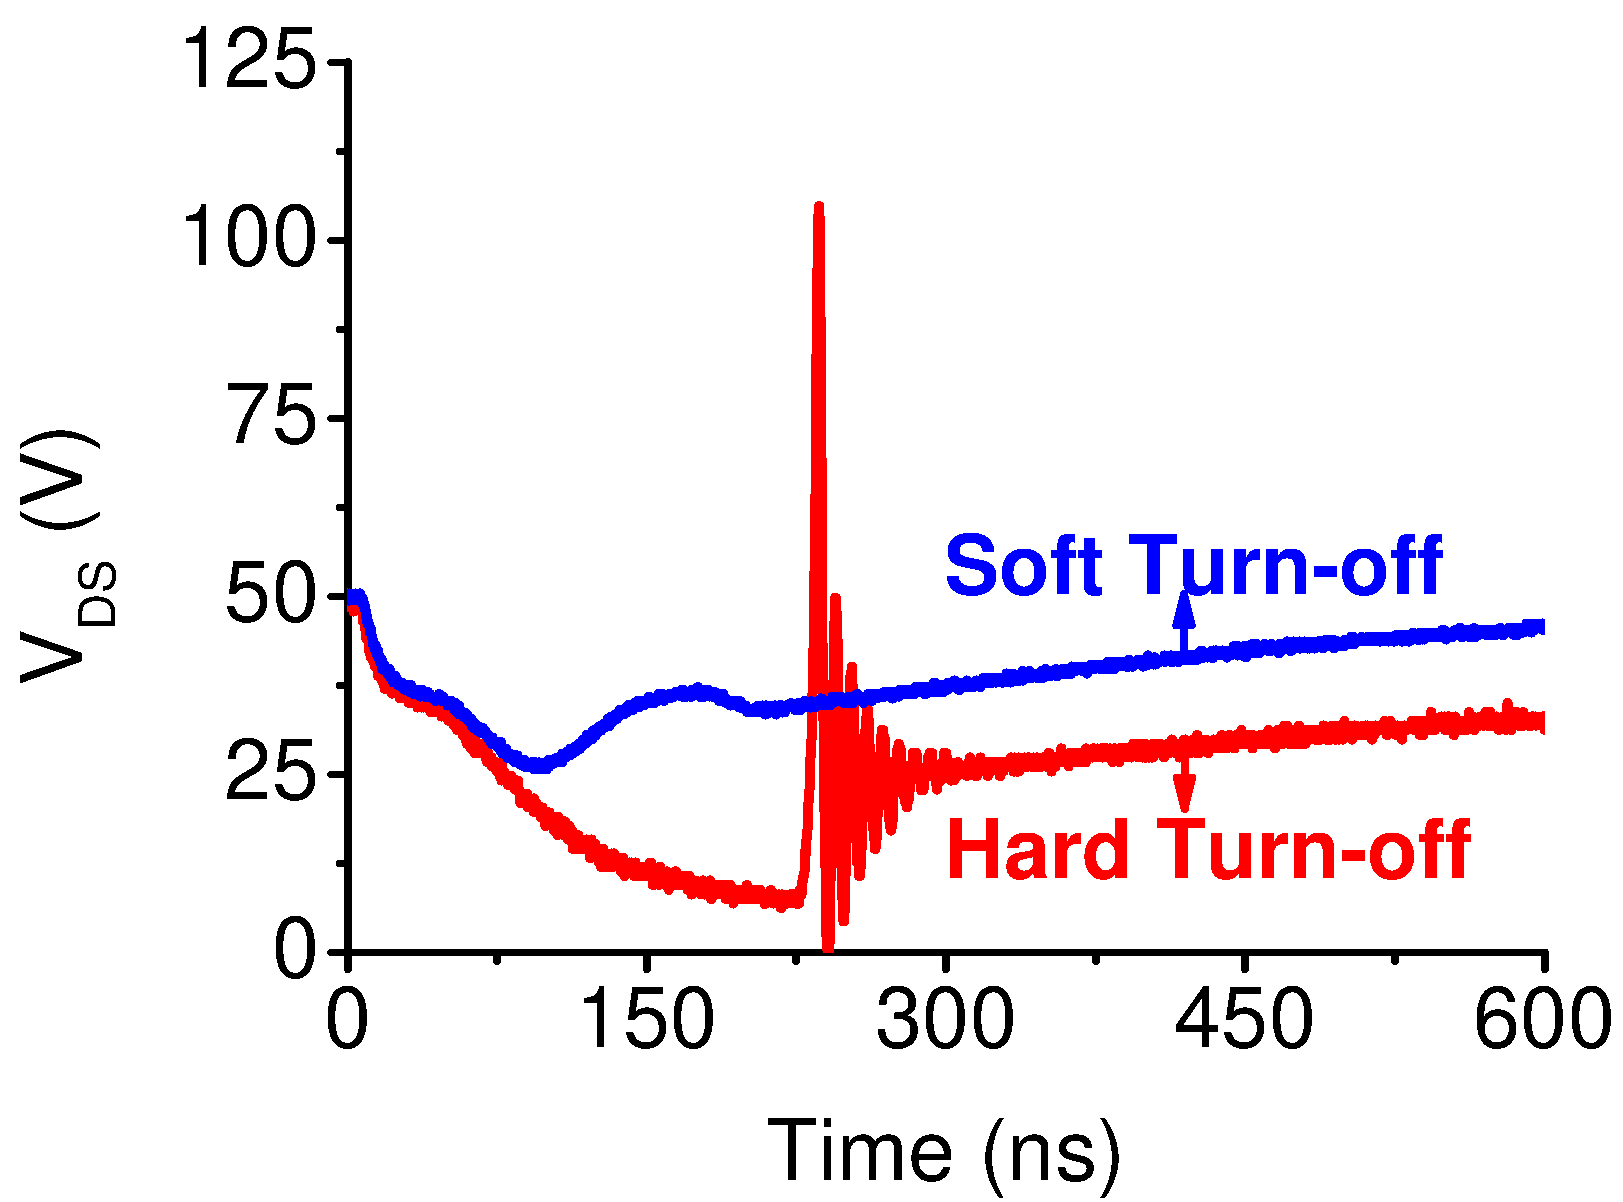
\includegraphics[width=2in]{Figures/Fig13-STOvsHTO.pdf}
\caption{Bottom side transistor drain-source voltages for hard and soft turn-off situations under 50 V DC bus voltage SC test}
\label{fig_hstoff}
\end{figure}
%%%%%%% Figure ends %%%%%%%

Furthermore, the robustness and the reliability of the proposed protection technique can be evaluated in two ways. Firstly, the SC protection mechanism must generate a response to an actual short circuit fault and secondly, the protection mechanism should not be triggered by a normal switching operation. Therefore, the filtered form of induced voltage ($V_{filter}$) during a SC fault and Double Pulse Test (DPT) are measured under different bus voltage levels and load currents as given in Fig.~\ref{fig_scp_vfiltouts}. All bus voltage levels result in the same amount of voltage induction for SC fault because the transistor current gets in saturation for all voltage levels which means the same trans-conductance for all voltage levels. These results also highlight the SC fault detection range. The SC fault can be detected as long as the bus voltage is high enough to bring transistors in saturation. In addition to SC fault results, the SC protection mechanism is not triggered in a DPT even for 400~V and 40~A of operation.

%%%%%%% Figure begins %%%%%%%
\begin{figure}[]
\centering
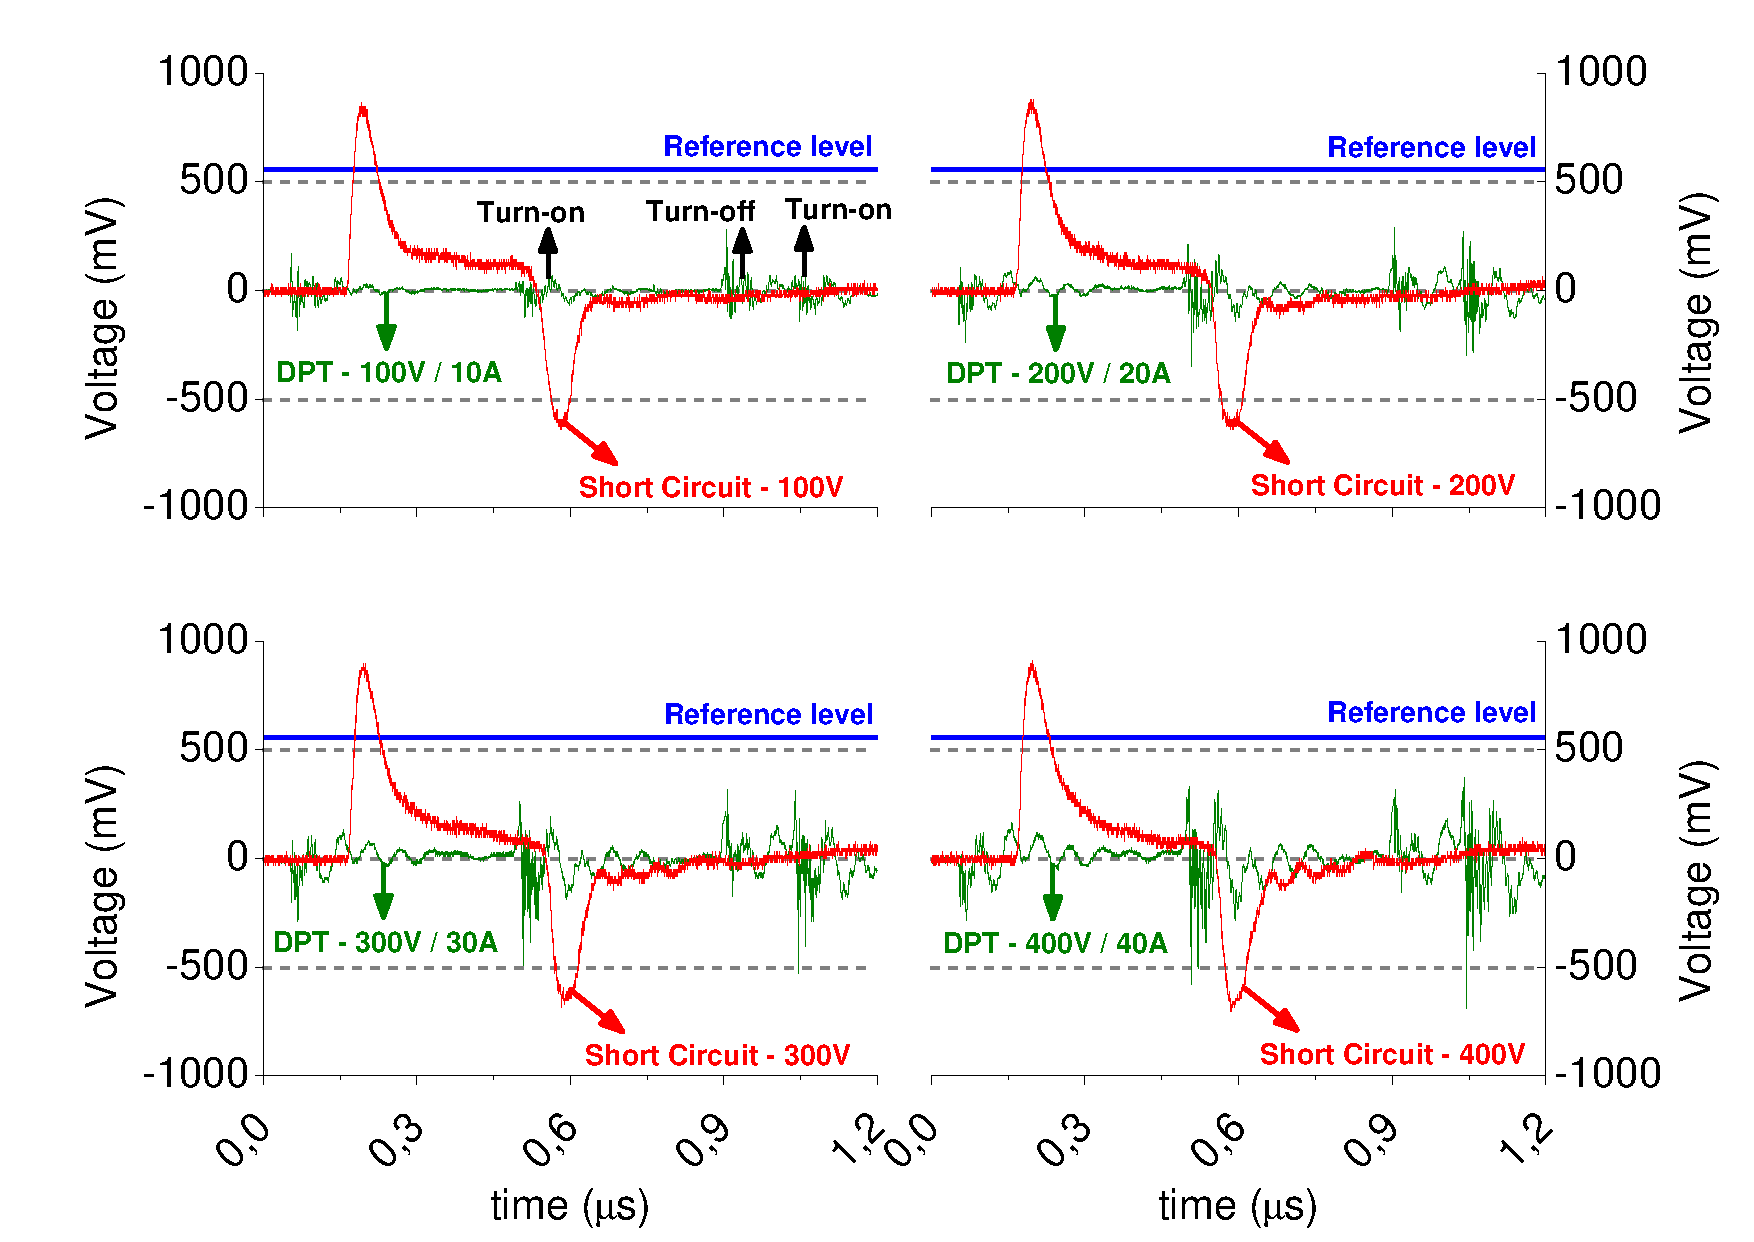
\includegraphics[width=3.4in]{Figures/Fig14-DPTandSCPVfiltouts.pdf}
\caption{Low-pass filter output voltage (V\textsubscript{filter}) for Double Pulse Tests (DPT) and HSF type Short Circuit (SC) faults under varying DC bias levels and load currents}
\label{fig_scp_vfiltouts}
\end{figure}
%%%%%%% Figure ends %%%%%%%

%%%%%%% Figure begins %%%%%%%
\begin{figure}[]
\centering
\includegraphics[width=3.4in]{Figures/Fig15-MPT.pdf}
\caption{Multi Pulse Test (MPT) waveforms: applied pulses to the gate-source terminals of control~\&~synchronous switches,  the load current~\&~voltage waveforms and filtered form of induced voltage (V\textsubscript{filter}) and reference level (V\textsubscript{ref})}
\label{fig_switching_ton}
\end{figure}
%%%%%%% Figure ends %%%%%%%

Besides SC fault results, multi pulse test (MPT) results are presented in Fig.~\ref{fig_switching_ton}, for 400~V and 40~A to show robustness of the SC protection mechanism and effectiveness of layout design. Since the designed bi-directional DC/DC converter utilizes quasi-square wave zero voltage switching, it applies a soft switching and voltage and current transitions are smooth. Therefore, the converter operation does not create high stress over SC protection mechanism. In order to show the reliability and robustness of the proposed SC protection technique, a multi pulse test is performed under 400~V. The inductive load current is charged up to 40~A with 160 pulses having 1.56~MHz switching frequency. Transistors are switched with 20~$\Omega$ and 2~$\Omega$ turn-on and turn-off gate resistances causing 60.2~$kV/\mu s$ and 96~$kV/\mu s$ maximum transition speed, respectively. In Fig.~\ref{fig_switching_ton}, V\textsubscript{gs} and V\textsubscript{ds} waveforms are shown for parallel control switches and parallel synchronous switches. The waveforms show that parallel GaN HEMTs turn on and turn off simultaneously and indicates the careful and proper layout design. Moreover, the V\textsubscript{gs} levels does not exceed the transistor threshold level, 1.7~V as a result of a false turn-on. This verifies the proper gate loop design as well. Lastly, the filtered form of induced voltage (V\textsubscript{filter}) is also presented in full view and zoomed view. The filter output voltage increases with increasing load current; however, it does not exceed the reference level and does not cause any mistrig.

In order to see the noise immunity better, the FFT results are given in Fig.~\ref{fig_fft_dptvsscpExp} where FFT results of induced voltage (V\textsubscript{sense}) and its filtered form (V\textsubscript{filter}) are compared for normal switching and under SC fault. The oscillating switching current acts as a very strong and close EMI source against SC protection mechanism. As explained in Section~\ref{sec_filterdesign}, the normal switching current carries more high frequency components but SC fault dominates for frequencies lower than 25~MHz in experimental results as well. These results also validate the filter design. Lastly, since the normal switching oscillations does not cause a mistrig, this highlights the robustness of the SC protection against other possible external EMI sources as well. However, a proper shielding would guarantee the safe operation for much noisy environments.

%%%%%%% Figure begins %%%%%%%
\begin{figure}[]
\centering
\includegraphics[width=3.4in]{Figures/Fig16-FFT_DPTvsSCPExp.pdf}
\caption{Comparison of FFT plots of induced voltage (V\textsubscript{sense}) and its filtered form (V\textsubscript{filter}) under SC fault and for normal switching conditions}
\label{fig_fft_dptvsscpExp}
\end{figure}
%%%%%%% Figure ends %%%%%%%

\section{Practical considerations}
Even though the proposed method utilizes the layout parasitics, the method should be able to tolerate variations of these parasitic components for practical applications. For this purpose, the effect of the sense loop's position with respect to the power loop on mutual inductance is analyzed by ANSYS Maxwell 3D. For the given layout design in Fig.~\ref{fig_pcbfea}, the sense loop is moved on two different axes and the change in the induced voltage is plotted in Fig.~\ref{fig_displacement}. The reference voltage level (V\textsubscript{REF}) is kept constant as in Fig.~\ref{fig_timing}, which can tolerate 30\% drop in the mutual inductance. If the drop in the mutual coupling exceeds 30\%, the SC fault cannot induce enough voltage to trigger the SC protection mechanism, which requires a reference level adjustment. Based on the results shown in Fig.~\ref{fig_displacement}, the mutual inductance can tolerate $\pm$ 2~mm variation on the Y axis, which is in parallel with the main current flow direction on the power loop. Conversely, the mutual coupling is sensitive to any displacement greater than 0.3~mm on the X axis, which is perpendicular to the main current flow direction on the power loop and does not provide a wide tolerance range. Although this margin seems low, PCB manufacturing techniques are accurate enough to prevent mutual coupling differences between mass-produced boards. Even though the most accurate results can be obtained by FEA analysis, it is not a must during the design stage. The rule of thumb is to keep the sense loop as wide as the power loop and to place it as close as possible to the power loop. Then, the reference level can be tuned according to the induced voltage. As each design requires verification of onboard functions, the SC protection can be verified during the adjustment procedure of the reference voltage level. Fortunately, this proposed method does not necessarily require a parasitic inductance modeling or characterization and the reference voltage level (V\textsubscript{REF}) can be adjusted practically by following these steps. Firstly, after verifying the soft turn-off (STO), an intended SC fault can be created by turning on high and low side switches at the same time, with a high enough DC link voltage to put the GaN HEMTs into saturation region (i.e. $\geq$100~V). Even though the SC protection circuit does not get a trigger signal during this tuning procedure, the SC fault has to be removed manually by the micro-controller with an STO after $\sim$75~ns in order not to risk a device failure. The low-pass filter output voltage (V\textsubscript{FILTER}) can be recorded by an oscilloscope. Then, the reference voltage level (V\textsubscript{REF}) can be set to $\sim$80\% of the peak level of the filter output. This experimental procedure enables the designer to test the performance of the SC protection circuit and to adjust the reference voltage level without modeling the layout parasitics.

%%%%%%% Figure begins %%%%%%%
% Bu figürde vectors çizilidir
\begin{figure}[]
\centering
\includegraphics[width=3.4in]{Figures/Fig17-Symbolic Layout-v2.pdf}
\caption{Variation of the induced voltage when the position of the sense loop changes with respect to the power loop}
\label{fig_displacement}
\end{figure}
%%%%%%% Figure ends %%%%%%%

\section{Discussions on Protection Circuits for Parallel Connected GaN HEMTs}

\begin{table}[t]
\renewcommand{\arraystretch}{1.3}
\caption{HSF Type SC fault response speed of different protection methods applied on GaN HEMTs}
\label{table_comparison}
\centering
\begin{tabular}{|c|c|c|c|}
\hline
Literature & Response Speed - Type & Sense Technique & Connection\\
\hline
\cite{Hou2019} & 70 ns - STO & $V_{DS}$ (2) & Single\\
\hline
\cite{Alemdar2019} & 80 ns - STO & Layout (3) & Single\\
\hline
\cite{Hou2018a}& 85 ns - STO & $V_{DS}$ (2) & Single\\
\hline
\rowcolor{Gray}
This work & 99 ns - STO& Layout (3) & \textbf{Parallel}\\
\hline
\cite{Dusmez2018} & 100 ns - HTO & Integrated (1) & Single\\
\hline
\cite{Wu2020} & 110 ns - HTO& $V_{DS}$ (2) & Single\\
\hline
\cite{Lyu2020} & 200 ns* - STO& $V_{BUS}$** (4) & Single\\
\hline
\cite{Gui2018} & 200 ns*** - HTO& $V_{DS}$ (2) & \textbf{Parallel}\\
\hline
\end{tabular}
\begin{flushleft}
(*) Response speed is measured by the author using the waveforms presented in the paper.

(**) Bus voltage is measured between positive and negative terminals of bus capacitor.

(***) The fastest response time is reported as 200~ns whereas the worst-case turn-off time is reported as 500~ns.
\end{flushleft}
\end{table}

%%%%%%% Figure begins %%%%%%%
\begin{figure}[]
\centering
\includegraphics[width=0.35\textwidth]{Figures/Fig18-SenseOptions - v2.pdf}
\caption{Different proposed sense techniques applied on GaN HEMTs to detect SC fault}
\label{fig_senseopt}
\end{figure}
%%%%%%% Figure ends %%%%%%%


SC faults can be sensed with different methods such as device integrated over current protection, drain-to-source voltage (V\textsubscript{DS}) measurement, sensing the induced voltage due to layout parasitics, or change in the bus voltage (V\textsubscript{BUS}). Those different sense techniques are shown on Fig.~\ref{fig_senseopt} as if they are applied on a parallel configuration. SC protection methods in literature and their performance are compared in Table \ref{table_comparison}. The response time of protection methods is taken as common measure. Based on the proposed protection solutions, soft turn-off (STO), i.e. gate clamping, activation or hard turn-off (HTO) activation is listed. STO activation period is an important measure since it determines the duration of uncontrolled SC current rise. However, if the proposed method does not include an STO mechanism, the initiation of HTO is taken as the comparison parameter. Even though, there are different protection types in literature, only the solutions applied on GaN HEMTs are compared in Table~\ref{table_comparison}.

All of the reported studies are able to get SC current under control in less than 500~ns which is the critical limit for GaN HEMTs with 350~V or more DC bus voltage \cite{Lyu2020}. First five solutions in Table \ref{table_comparison} are able to activate STO in less than 100~ns with 30~ns deviation as maximum. The proposed SC protection mechanism in this paper is designed and verified for parallel connected GaN HEMTs and it starts STO in 99~ns and fault is removed completely in 250~ns in total.

The sensing methods other than the method proposed in this paper (3 in Fig. \ref{fig_senseopt}) might not be easily adapted to parallel configuration for several reasons. The integrated protection design comes together with the monolithic gate driver structure which disables the device paralleling due to the risk of unequal propagation delay of embedded gate drivers of paralleled switches. Moreover, integrated protection technique is built without an STO mechanism and cannot be modified by the designers. The second method, V\textsubscript{DS} sense, is applied on many designs for single bridge connection and also for the parallel connection \cite{Gui2018} as well. The reported response times in \cite{Gui2018} are 200~ns for the fastest response and 500~ns for the slowest response. As mentioned earlier, 500~ns is the critical duration for an application with a voltage bias higher than 350~V. Additionally, it is also reported in \cite{Wu2020} that the GaN HEMTs get damaged after around 200~ns with 400~V bus voltage and 6~V gate voltage for GS66508T, which is the same transistor used in this study. The third method, sensing the induced voltage created by the power loop current, is successfully applied on single and parallel connected configurations. The response time is faster than 100~ns for both configurations. Lastly, the bus voltage sensing is a method that could be applied on parallel configuration. The main concern regarding this method is that currently there is no reported solution faster than 200~ns, and this solution gives the slowest response time in general (200~ns for GaN HEMTs \cite{Lyu2020}, 224~ns for GaN GITs \cite{Wang2019}).

Moreover, short circuit protection for a parallel bridge configuration is more challenging than single bridge configuration. Firstly, the layout design considerations of parallel connected transistors are different than single bridge designs. Even though both designs aim to minimize the gate loop and power loop inductances, it is also essential to have equal layout inductances for parallel connected transistors \cite{Lu2017a}, which is critical to achieve simultaneous switching of the parallel connected transistors. Instead of placing the gate driver as close as possible to the GaN HEMT as in single configuration, the gate driver has to be placed between parallel connected GaN HEMTs, which results in higher gate loop inductances. This requires either slowing down the parallel GaN HEMTs \cite{Reusch2016} or risking higher oscillations on the gate-source voltage. An oscillation on the gate-source voltage causes oscillation on the device current during the normal switching operation. Therefore, in order to eliminate the mis-trigger on SC protection circuit, the filter has to be quite tight, which slows down the response time of protection circuit. This fact is actually verified by the studies presented in Table~\ref{table_comparison}. For both  V\textsubscript{DS} sensing and layout sensing methods, the response times  of protection circuit is slower for parallel switch configuration. Fortunately, the response time of the proposed method is 99~ns for parallel operation with only 19~ns additional span in comparison to \cite{Alemdar2019}.

Secondly, the protection methods, which are based on sensing device characteristics, as in V\textsubscript{DS} sense, require short connection to device terminals. However, considerably large discrete protection circuits complicate the power loop and the gate loop layout design \cite{Hou2019}. Therefore, in order to increase the flexibility in the design of power loop and the gate loop, the dual-gate pads structure of some GaN HEMTs are utilized in a way where one of the gate pad is used for gate driver and other one is used for the protection circuit \cite{Hou2019}. However, this cannot be realized with parallel configuration, since the gate pads of transistors are utilized for the gate driver. Thankfully, the layout based sense method does not require to be placed closely to GaN HEMTs, which relaxes the space limitations on PCB board. The proposed design is a good example of space utilization with integration of SC protection method for parallel switches. An evaluation half-bridge board (GS66508T-EVBDB2) is designed by the manufacturer for GS66508T, which has 35 mm height and 85 mm length without a protection circuit \cite{GaNSystemsInc.2020}. Similarly, the proposed design in this paper has 40 mm height and 90 mm length but also with double current carrying capability and integrated SC protection. Therefore, the layout based SC fault sense method does not necessarily bother designers with space limitations, and compact solutions could be obtained without deteriorating the power loop and the gate loop.

Up to now, there is only one example for SC protection of parallel connected GaN HEMTs, which applies the desaturation technique \cite{Gui2018}. The main advantage of the desaturation technique is to detect both HSF or FUL type SC faults. However, based on the proposed protection methods focusing on parallel GaN HEMTs as presented in Table~\ref{table_comparison}, the response speed of the desaturation technique is lower than the layout based protection technique. An experimental comparison results were provided in \cite{Awwad} for the desaturation technique and layout parasitics. It is shown that the layout parasitics method is faster than the desaturation technique \cite{Awwad}. Though the layout based sense method is only able to detect HSF type SC faults, the FUL type SC faults can be detected by using current sense structures already employed by the current mode controller. Moreover, even though the redundancy can be increased for desaturation technique by applying the protection scheme to each individual paralleled GaN HEMTs, it is not practical due to increased cost and space limitations on the PCB.

Considering all the proposed protection methods in the literature for HSF type SC fault, two suitable techniques can respond to a SC fault of paralleled GaN HEMTs. A desaturation technique applied on a parallel connected GaN HEMTs is demonstrated in \cite{Gui2018} and the layout sensing technique applied on paralleled GaN HEMTs is proposed in this paper. In comparison to single half-bridge design, parallel connected GaN HEMTs require a more sophisticated layout design, so it narrows down the flexibility of space utilization on a printed circuit board. It is shown that the layout based sensing method does not deteriorate the circuit layout and a high frequency switching performance above 1.5~MHz  at 400~V DC link level can be obtained without causing a mistrig. The proposed half-bridge board, distinctively including the SC protection circuit, has similar dimension lengths with industrial boards. Furthermore, the response time of the proposed method is 99~ns which is lower than other proposed techniques applied on parallel connected GaN HEMTs. As a result, layout based protection technique has a proven capability of reacting against the SC fault of a parallel connected GaN HEMTs under 100~ns where the GaN HEMT stays healthy for 200~ns \cite{Wu2020} during the HSF type SC fault.


\section{Conclusion}

In this paper, a short-circuit protection method based on sensing the voltage created by high $dI/dt$ of SC current is applied on a parallel switch half-bridge. The implementation of short-circuit protection technique on a parallel configuration is different than a single bridge configuration due to symmetric layout design constraints. The reported SC protection methods in the literature are evaluated and compared for parallel configuration. The proposed layout based SC protection method is advantageous for parallel configuration because the sense circuit does not have to be placed close to a transistor or a half-bridge which relaxes the space limitations and increases the flexibility for symmetric layout design.

Experimental results show that short circuit protection mechanism is able to detect the fault in 40~ns. After detecting the fault, a soft turn-off process is initiated within 100~ns to keep transistors in safe-operating-area. Short circuit fault is completely removed in 250~ns as a final step. Moreover, experimental results also show that proposed method does not distort the power loop or the gate loop layouts. As a result of optimized layout design, gate voltage is not distorted by the miller capacitance which could have initiated a short-circuit fault easily. The reliability of the proposed SC protection method is tested by a multi pulse test conducted with 160 pulses at 1.56 MHz switching frequency.

The proposed board can be adapted to many applications with increased current capability by paralleling and with its short-circuit protection ability.

\section*{Acknowledgment}

The authors would like to thank Enes Ayaz, Furkan Tokgöz, Gökhan Çakal and Nail Tosun for their valuable support.

\ifCLASSOPTIONcaptionsoff
  \newpage
\fi

\bibliographystyle{IEEEtran}
\bibliography{Device-2020-Feb.bib}
\end{document}


